\section{Desired model}

\begin{figure}[tb]
	\centering
	\includegraphics[width=\linewidth]{desiard_model.eps} 
	\caption{Performance model}
	\label{fig:performance_model}`
\end{figure}

As the topology of any future \xcloud and forthcoming proposed mobile networks is yet to be determined, in this paper we propose a generic telecom infrastucture model that disregards from specific generational properites such as the physical layer and cell load-balancing. Nevertheless, conceivably and in order to confine the geographic domain of the model it adheres to current LTE cell plannig pracices. 

In order to explore the fundamental dynamics of the generic case, as such, the model does not adhere to any soci-demographic patterns or urban topologies. The mobile network base tstaions are therefore uniformly distributed across its 2-dimensional domain.

Similarly, in order to represent the breth of possible services, the service model needs to generate traffic that is characteristic of a generic \ue. Additionally, the generated traffic needs to be provided by a stochastic process that is indepedant of location.

The concert of the mobility model and the service model in a uniformly distributed mobile network will provide the modeled \dcs with relevant request patterns. It is worth reitterating that the traffic load is more relevant to our investigation than specific topological and network properties.

The \dc model will host multiple VM that will process the arriving requets corresponding to its service commitment. Additionally when a VM is migrated between \dcs it shall incurr a load on the both \dcs.